\documentclass{vldb}

\usepackage{graphicx}
\usepackage{listings}
\usepackage{subcaption}
\usepackage{caption}
\usepackage{hyperref}
\lstset{
  language=C,
  basicstyle=\ttfamily\scriptsize,
  tabsize=2,                    % sets default tabsize to 2 spaces
%  columns=flexible,
  xleftmargin=18pt,
  xrightmargin=1em,
  numbers=left,
  numberstyle=\scriptsize,
  numbersep=1em,
  showstringspaces=false,
  alsoletter={-},
	morekeywords={todo}, %FIXIT
	otherkeywords={TD},  %FIXIT
  captionpos=b,
  escapeinside={@}{@},
  commentstyle=\color{gray},
}


\begin{document}

\title{Incremental Memory Footprint Estimation for MonetDB}

\author{Pavlos Katsogridakis, Ying Zhang, Martin Kersten}

\maketitle

\begin{abstract}
Estimating the memory footprint of a query is an important
feature for a database system. It can answer the question whether
a query will fit in memory, and also gives the compiler the opportunity
to perform a lot of optimizations.
In this document we present Malcom (Mal ALgebra COst Model), a memory footprint
estimator, that incrementally builds a memory cost model for MAL instructions,
based on previous query executions. We evaluated our system using the tpch
benchmark suite, and a real world air traffic dataset.
\end{abstract}

\section{Introduction}
\label{Introduction}
Since its inception, database designers have keenly looked at the opportunities to use large,
distributed processing platforms. Cluster-based products are readily available \cite{},
but are often limited to a few tens of compute nodes and call for a strong engineering
to avoid hardware bottlenecks, such as in Exadata \cite{}, SQL PWD \cite{}, IBM Blu \cite{} and ....

A plethora of research activities have showen that in all but the simplest cases,
achieving a good performance is at least very hard. Especially when a query
involves joins spread over multiple compute nodes and requires expensive data exchanges.

The predominant way out, taken in NoSQL systems  \cite{Casandra,Impala}
is to address part of the problem space by focusing on select-aggregate queries.
This focus on part of the problem space for distributed query processing has
been pivotal to support big-data analytics in many real-world circumstances,
as shown by the rapidly growing popularity of Spark \cite{},
which is widely used nowadays to encode distributed applications.
The basic abstraction in Spark is a Resilient Distributed Dataset (RDD),
which represents an immutable partitioned collection of elements that can be
operated on in parallel using operators, such as map, filter, persist and aggregates.
Moreover, the RDD is the basic component to exchange between
operators, threads, cores and machines.
In essence, an RDD can be seen as a relational table used for interoperability,
an approach that can be traced back to Microsoft's ODE \cite{} used for decades
to exchange data between DBMS and applications. Similar functional abstractions
can nowadays be found in R's Dataframes \cite{} and Python Pandas\cite{}.

%explain resident/resilient, the former tells it can be re-constructed upon need.

Although in most cases, it is easier to scale-up for improved response time,
partitioning a database to benefit from the low price tag, better use of parallel IO,
or resource limitations of smaller machines is still worth considering.
Distributed database management systems have followed the same route \cite{distributed DB}.
However, the major hurdle that has blocked the progress for decades is the insurmountable task
to create an optimizer to derived an optimal plan \cite{}.

In this paper we take a fresh look at optimizing query processing in the context
of where intermediates in a query plan are fully materialized before passing on
towards the next operator. This model fits the Spark programming model,
but also the query execution model underlying MonetDB.
Resilient intermediates provides new avenues for query optimization and
scheduling as its underlying computation model is based on
materialization of all intermediate steps.

The main contributions of this paper are
\begin{itemize}
	\item we develop a simulator to predict size and processing bounds for queries based on resident intermediates.
	\item We provide a novel optimizer to minimize memory footprint and processing time
	\item We demonstrate the approach is robust against varying data distributions.
	\item We demonstrate the quality of our approach using an extensive evaluation against TPC-H and real-world databases.
	\item ...
\end{itemize}

The approach taken differs from traditional Cost-Based Optimizers (CBO), which generally sample the state of actual execution of primitive operations, e.g. Oracle CBO\footnote{\url{https://docs.oracle.com/cd/B10500_01/server.920/a96533/optimops.htm}} and HIVE CBO\footnote{\url{https://hortonworks.com/blog/hive-0-14-cost-based-optimizer-cbo-technical-overview/}}, because after each query step we have precise knowledge of the resources claimed.
Malcom harvests this information to predict future operations of similar nature.
The rational stems from the common knowledge that many database application
environments have a limited number of ``business transactions'' or ``BI templates'' where only some parameters are changed with each call.
This knowledge has been used in the past to, for instance, drive development of DBA wizards\footnote{E.g. MicroSoft AutoAdmin: \url{https://www.microsoft.com/en-us/research/project/autoadmin/}} for index selection and self-tuning optimizers \footnote{E.g. IBM DatArces Optimizer: \url{https://www.ibm.com/us-en/marketplace/datarcs-optimizer}} to avoid expensive join paths.

Outline of paper. Section \ref{Background} provides a short introduction
to the MonetDB architecture and the projects involved.

\subsection{Use Cases}
\begin{enumerate}
  \item Prediction of the memory footprint
  \item Instruction ordering by the compiler
  \item Parallelism level
  \item Join dictionary build
\end{enumerate}

\section{Background}
\label{Background}
In this section we summarize the salient features of resilient intermediates
for query processing., the leading open-source column store and the envisioned
system ExaNest, an exascale HPC platform for data-intensive computing.

\subsection{A Column Store}
%Recap some MonetDB stuff on how queries are compiled.
MonetDB is a widely used column store that internally uses resident
intermediates to break up query processing in well identified steps.
The query plan is broken up into independent steps, glued together into a
dataflow dependency graph. The dataflow graph is greedily consumed by the
database kernel assigning a single core to a single operation.
The resource pressure is kept at a minimal to trim down the degree of parallel
processing when the main resource, RAM, is heavily used.
The system can be instructed to produce an event record for each completed instruction.
This provides a.o. insight into the input/output sizes and timing.

\subsection{Distributed Query Optimizers}
% summarize
The predominant scheme to scale out database processing is to break the base
tables into independent partitions using either a hash-key or ranges.
The partitioning scheme can be used to orchestrate distributed processing
in an optimal way most of the time.

Apache Spark CBO\footnote{\url{https://databricks.com/blog/2017/08/31/cost-based-optimizer-in-apache-spark-2-2.html}}: add some description


\begin{figure}[!htb]
  \centering
  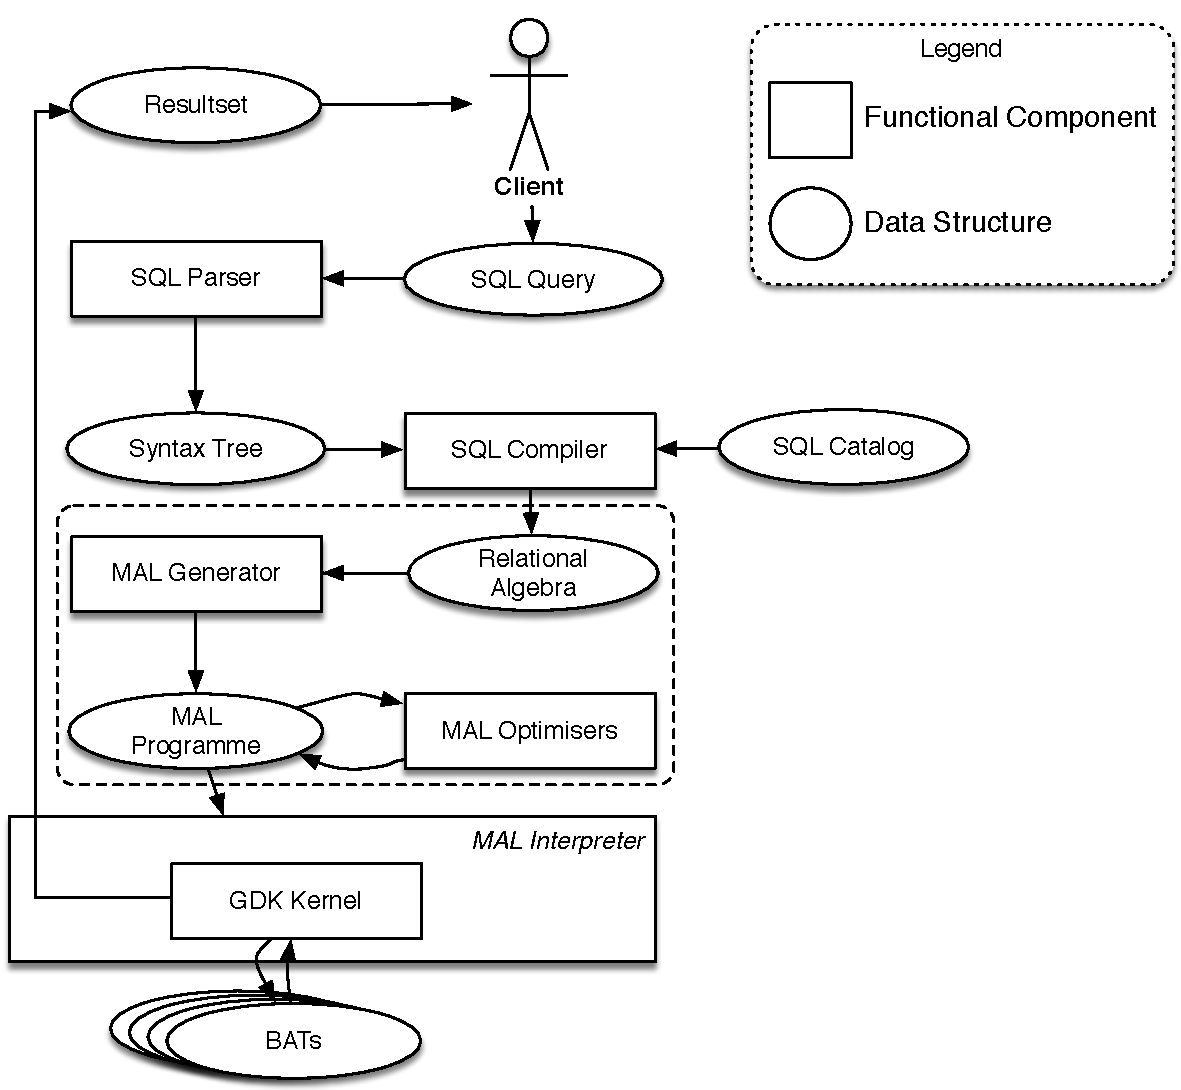
\includegraphics[width=0.9\columnwidth]{figs/MDB_architecture.pdf}
  \caption{MonetDB implementation architecture}
  \label{fig:mdbarch}
\end{figure}

\section{MonetDB Query Execution Model}
In this section we describe how the MonetDB query execution engine was used
 to develop a novel .... We also illustrate the data at our disposal to predict

\subsection{Architecture}
Figure \ref{fig:mdbarch} illustrates the components our reference system, MonetDB,
to execute an sql query. The SQL Parser and MAL Optimisers deploy well-known
rewriting rules to reduce the intermediate sizes and processing time.
It does not rely on any cost-model or pre-computed statistics
(aside from the whereabouts of the data partitions on separate nodes)

The middle layer (in the dashed box) is a sequence of specialized optimizers that morph the logical
plan received from the SQL compiler into a physical execution plan.
Constant expressions are evaluated, common sub-expressions are identified,
the dataflow graph for parallel processing is derived, etc.

The bottom layer (under the dashed box) contains the implementation of the relational operators.
Each operator takes as input the resident intermediates produced before
or accessing the persistent data on disk.
The actual implementation is often quite complex,
because each operator can be implemented in a multitude of ways.
Since the operator has full knowledge on the actual parameters,
it becomes easy to select the proper path.
Some operators even perform a sampling step before making a choice on the
 preferred algorithm.

To illustrate consider the following simple SQL query
The actual code executed by the MonetDB kernel is shown in Figure \ref{label}.
%clarify what you see

The details of the actual execution can be gathered using the Stethoscope.
A single record is shown in Figure \ref{}. Of interest to this paper are
the properties shown for the arguments and return variables.

\subsection{Profiling Information}
The MonetDB kernel can be instructed to emit profiling events.
Every primitive function comes with an event record taken at the start and
upon completion of the operation. The event record contains details on the
arguments passed, their type and size. Where ever possible the arguments
are linked with the underlying persistent column. Intermediate columns are
nameless and we only can rely on their type/cardinality.
Upon completion, we also know the exact size of the result and the time consumption.
Thread affinity is also available, but for the remainder of this paper ignored.

Explain a MAL instruction
For the remainder of this paper it is necessary to have a basic knowledge of the
MAL programming language in which all SQL queries are translated.
The MAL language is purely designed as intermediate language to express the operations.

The general format is
\begin{verbatim}
content...
\end{verbatim}
Every function belongs to a module. The arguments are either typed scalar
values (:type) or a reference to a column (:bat[:type]).

\section{Micro Models}
With an abundance of events we can start to derive models for each of the instructions.
A micro model is derived that can be used later for ease of simulation
alternative execution plans. We study them based on similar properties.

\subsection{Argument size}
When we try to predict an instruction, unless it is the first one,
we do not know exactly the argument size. So starting from the beginning,
we build a tree associating each variable to a prediction of the instruction it was produced,
so that we can use the predicted return size as input to the next instruction
we want to predict.

\subsection{Arithmetic Operations}
The operations can be grouped by complexity to predict the outcome of a hypothetical operation.
The first group includes the {\em batcalc} operations.
They all obey the following structure:
\begin{verbatim}
  res:bat[:lng]:= batcalc.==( l:bat[:lng],r:bat[:lng])
  res:bat[:lng]:= batcalc.==( l:bat[:lng],r::lng)
  res:bat[:lng]:= batcalc.==( l:lng,r:bat[:lng])
  res:bat[:lng]:= batcalc.==( l:lng,r:lng)

\end{verbatim}
The argument is either scalar or a reference to a column.
However, in all cases the number of result tuples can be looked up from the argument events.
The processing time depends mostly on the type's footprint and the influence of concurrent activity.


\subsection{Limit Operations}
Limit and sample operators(firstn, and sample? in MAL) are also trivial,
we just output the minimum of the argumens size and the limit size.


\subsection{Aggregate Operations}
This category includes operations like sum, avg, min, max, single, dec\_round
The count of the result is obviously one.

\subsection{Select Operator}
\subsubsection{Range Selects}
To predict the size of a range select, we used the kNN algorithm,
using k=5, to find the 5 closest selects to the one we want to predict,
considering the lower and higher bounds as distance metrics.
When we are facing a one bound select ($<$,$>$ etc) we use the
dataset statistics to fill the other bound (e.g in case of $<$ we want the column min).
\subsubsection{Point Selects}
Again we use the kNN to find the 5 closest points,
and extrapolate based on the argument size.

\subsubsection{Like Selects}
Future work :P

\subsubsection{Subsequent Selects}
%TODO make it more general
In case of intermediate select instructions, the ranges are not adequate to
make an accurate prediction, because the argument size may vary based on the
previous selects. To overcomes this we incorporated the estimations of the
previous intructions, to build a graph that relates each variable to a size
estimation. This way we cal also use the argument estimation to predict the
size of the select result. The code for selection prediction is shown at
Figure\ref{sel:code}. In real life it is very common to find correlated columns,
in which the first selection may affect non-linearly the second.
In our design we do not handle such cases(Future work).

\begin{figure}[t]
\begin{lstlisting}[frame=single]
  def div(i1, i2):
    return (i1.hi-i1.lo) / (i2.hi-i2.lo)

  def extrapolate(traini, testi):
      traini.cnt*div(testi,traini)*testi.approx_arg_cnt/traini.argcnt

  def predict(testi, traind, approxG):
    knn5 = traind.knn(testi,5)
    return sum([i.extrapolate(testi) for i in knn5]) / len(knn5)
\end{lstlisting}
  \caption{Code snippet for making predictions for range selects}
  \label{sel:code}
\end{figure}


\subsection{Join}
(Run a kNN(k=5) on the joins we have in our dictionary,
that operate on the same two columns if possible,
and find the ones closest based on the argument sizes).

\subsection{Grouping Operations}
The groupby signature is:
\begin{verbatim}
  (bat[:oid], bat[:oid], bat[:X]) := group.groupdone(bat[:X]);
\end{verbatim}
The first return value is the ids of the grouped column, the second is
the ids of the discinct values of the column(the third what ??). To predict
the size of the return variables, we use the ground statistics of the column
(size, count, discinct values).

Subgroupdone has a similar signature to groupdone, but it operates on intermmediate
variables, where we do not have the column information. In this case, we run a
kNN based on the argument sizes.

Orderby is translated into sort in MAL.
\begin{verbatim}
(bat[:X],bat[:oid],bat[:oid]) := algebra.sort(bat[:X], bat[:oid], bat[:oid], bit, bit)
\end{verbatim}
The size of each return value is exactly the same as the corresponding argument size.

\subsection{Set instructions}
We do not have any relevant information to do an accurate guess for the
set instructions, so we output the worst case of the result.
$$ intersect(A,B) ~= min(A,B)$$
$$ merge(A,B) ~= A+B $$
$$ diff(A,B) ~= A $$
% diff,union,intersect

\subsection{Load instructions}
\subsubsection{bind}
Bind instruction loads(or memory maps) a column into memory,
thus the result size is the size of the column.
\subsubsection{bind\_idxbat, tid}
Tid and bind\_idxbat do not produce any memory overhead

\subsection{Special cases}
\subsubsection{String similarity}
To predict a selection of a string column,
we used the levenshtein distance as a metric...
\subsubsection{Projection returning str}
In some weird cases, the projection instruction
returns str(copies from heap) instead of ids,
which makes hard to predict. In this case, we run a kNN
based on the type and argument distance, to find a similar
instruction use this to find the output size.

\begin{frame}[fragile]
\frametitle{Tpch sf10 Evaluation}
\begin{block}{}
\begin{itemize}
	\item Produce 200 queries randomizing the selection values
	\item Keep the original query as test set
	\item Error = 100 * (predict\_mem - real\_mem) / real\_mem
\end{itemize}
\end{block}
\end{frame}

\begin{frame}[fragile]
	\frametitle{Tpch sf10 Q6}
  \begin{figure}[t]
    \centering
    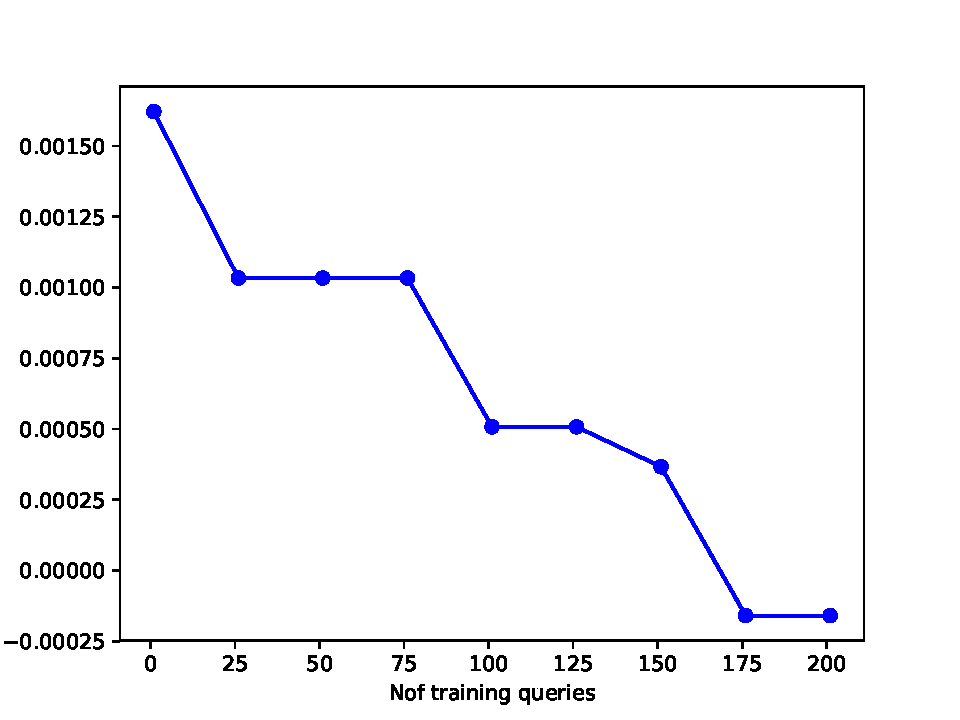
\includegraphics[width=1.0\textwidth]{../figs/tpch10/tpch10_q06_memerror.pdf}
		\caption{Relative Memory Error for query 6}
  \end{figure}
\end{frame}


\begin{frame}[fragile]
	\frametitle{Tpch sf10}
  \begin{figure}[t]
    \centering
    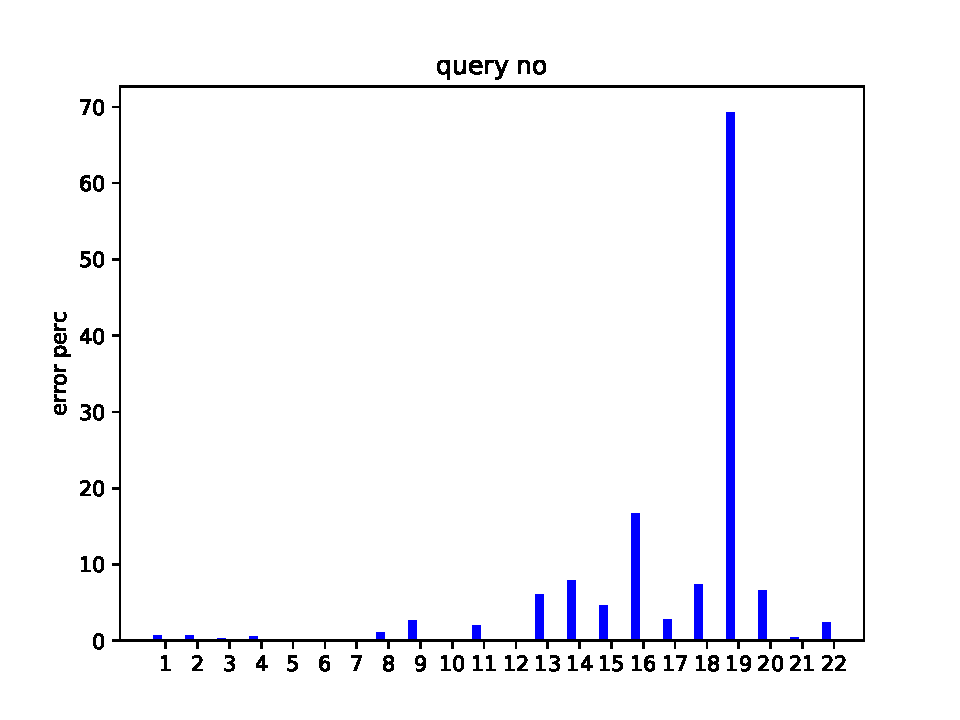
\includegraphics[width=1.0\textwidth]{../figs/tpch10/mem_error_1-23.pdf}
  \end{figure}
\end{frame}

\begin{frame}[fragile]
\frametitle{Airtraffic benchmark suite}
\begin{lstlisting}[basicstyle=\ttfamily\tiny, language=SQL,escapechar=!]
SELECT SQL_MIN("Origin", "Dest"),
       SQL_MAX("Origin", "Dest") AS route,
       COUNT(*) FROM ontime
!\colorbox{yellow}{WHERE 2010-09-11<FlightDate AND FlightDate<2011-09-11}!
GROUP BY route;
\end{lstlisting}
	\begin{figure}[!htb]
	    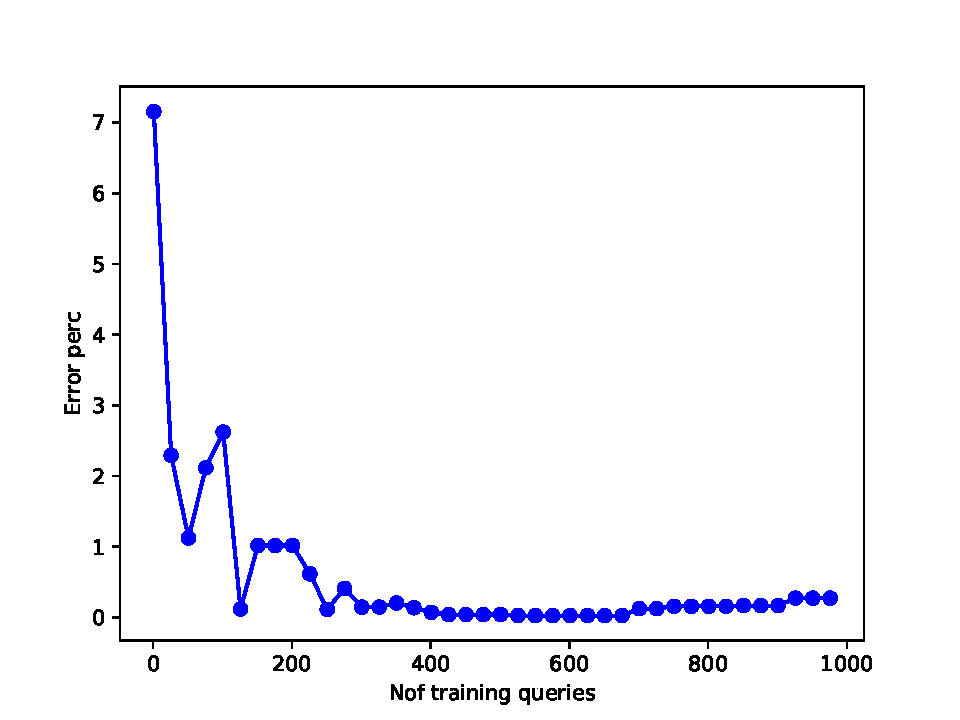
\includegraphics[scale=0.45]{../figs/airtraffic/airtraffic_sel11_error.pdf}
	    % \caption{Q11 select error}
	  % \begin{subfigure}[t]{0.4\textwidth}
	  %   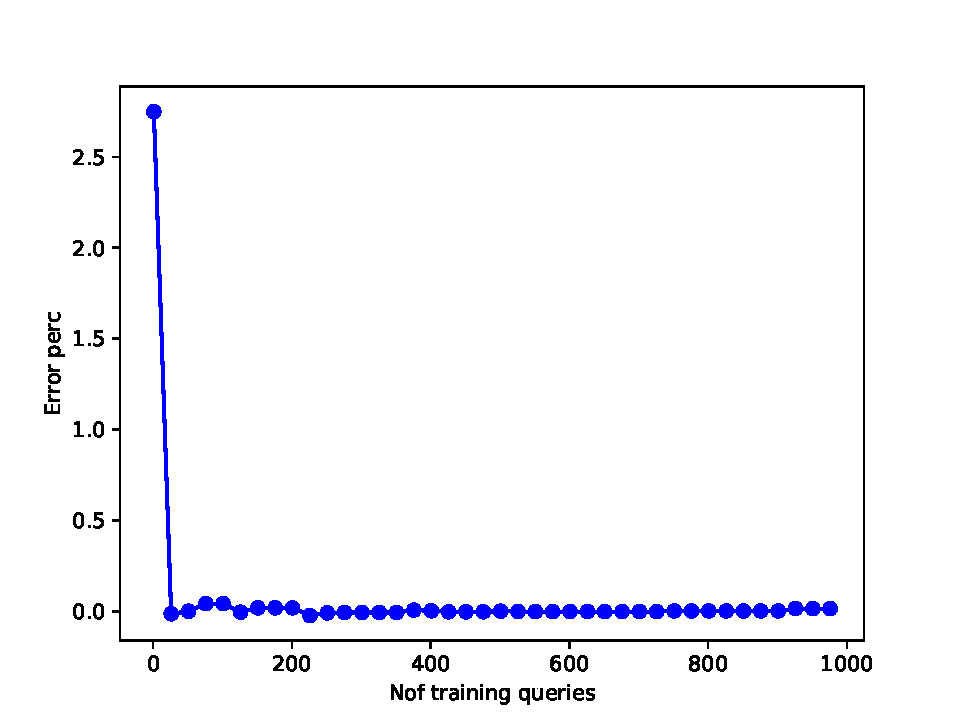
\includegraphics[scale=0.3]{../figs/airtraffic/airtraffic_q11_memerror.pdf}
	  %   \caption{Q11 memory error}
	  %   \label{fig:mem04}
	  %  \end{subfigure}
	\end{figure}
\end{frame}

\begin{frame}[fragile]
% \frametitle{Airtraffic benchmark suite}
\begin{lstlisting}[basicstyle=\ttfamily\footnotesize, language=SQL,escapechar=!]
SELECT "DayOfWeek", COUNT(*) AS "Flights"
FROM ontime
!\colorbox{yellow}{WHERE "DepDelay" > 15}!
GROUP BY "DayOfWeek"
ORDER BY "DayOfWeek";
\end{lstlisting}

	\begin{figure}[!htb]
	  % \begin{subfigure}[t]{0.4\textwidth}
	  %   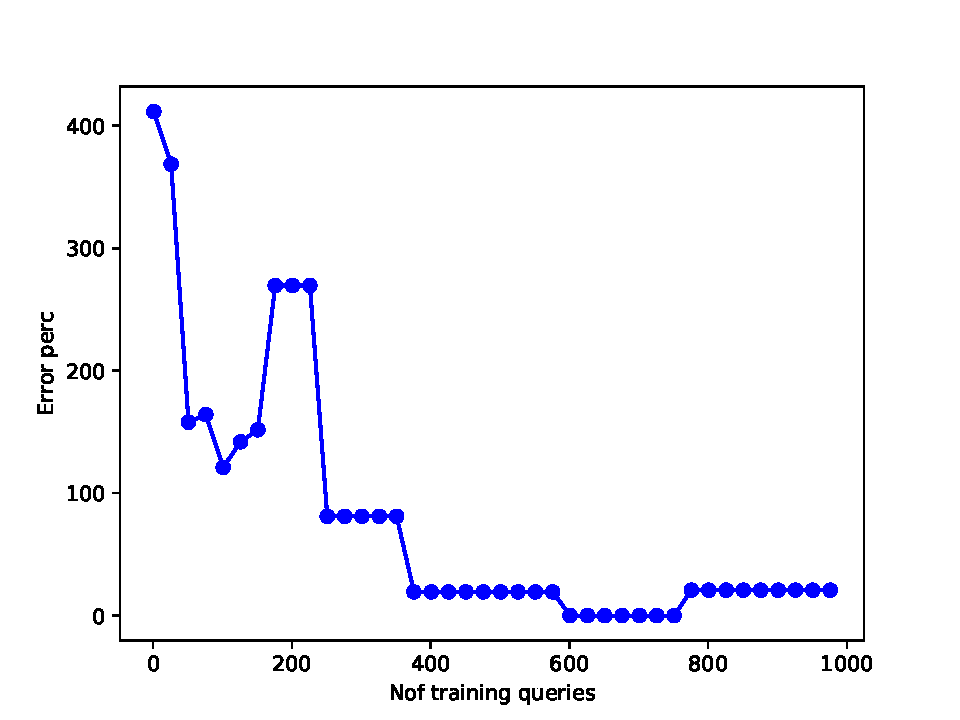
\includegraphics[scale=0.3]{../figs/airtraffic/airtraffic_sel04_error.pdf}
	  %   \caption{Q04 select error}
	  %   \label{fig:sel04}
	  % \end{subfigure}
	  % \begin{subfigure}[t]{0.4\textwidth}
		\centering
	  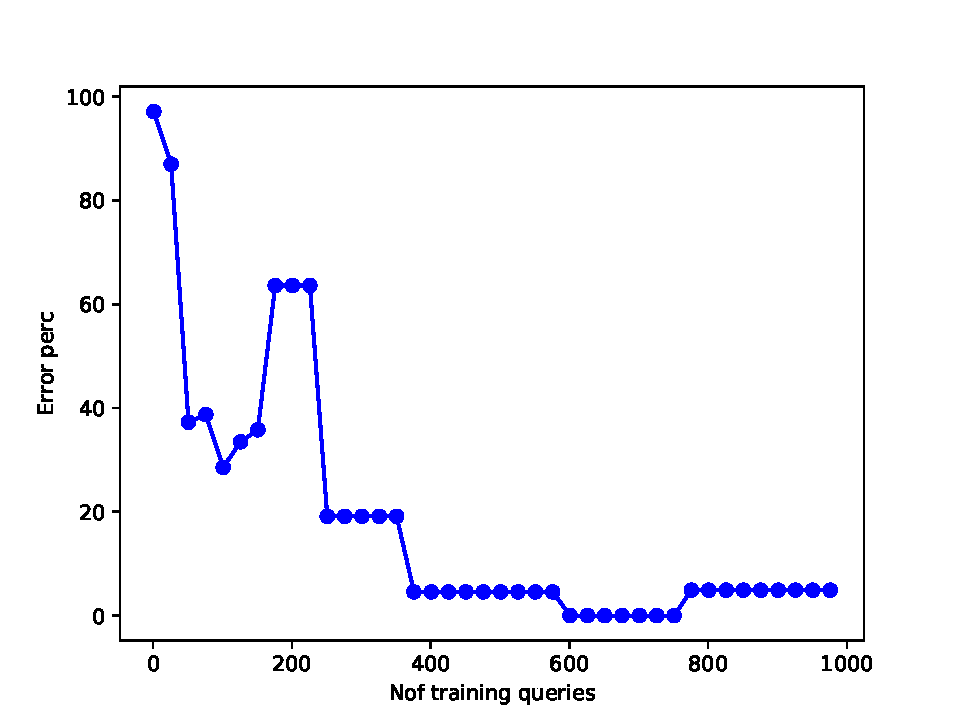
\includegraphics[scale=0.45]{../figs/airtraffic/airtraffic_q04_memerror.pdf}
	  \caption{Q04 memory error}
	    \label{fig:mem04}
	  %  \end{subfigure}
	\end{figure}
\end{frame}


\begin{frame}[fragile]
% \frametitle{Airtraffic benchmark suite}
\begin{lstlisting}[basicstyle=\ttfamily\footnotesize, language=SQL, escapechar=!]
SELECT "Origin" AS ap, COUNT(*) AS cnt_in
FROM ontime
!\colorbox{yellow}{WHERE "Dest" = 'ORD'}!
GROUP BY "Origin"
\end{lstlisting}
	\begin{figure}[!htb]
		\centering
		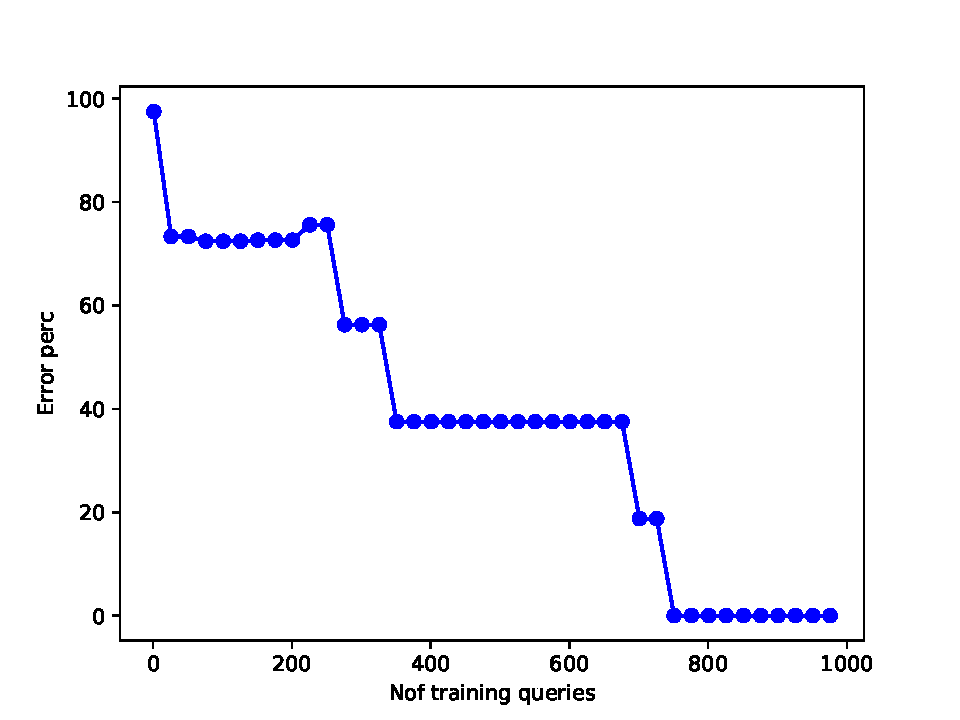
\includegraphics[scale=0.45]{../figs/airtraffic/airtraffic_sel10_error.pdf}
		\caption{Q10 select error}
	  % \begin{subfigure}[t]{0.5\textwidth}
	  %   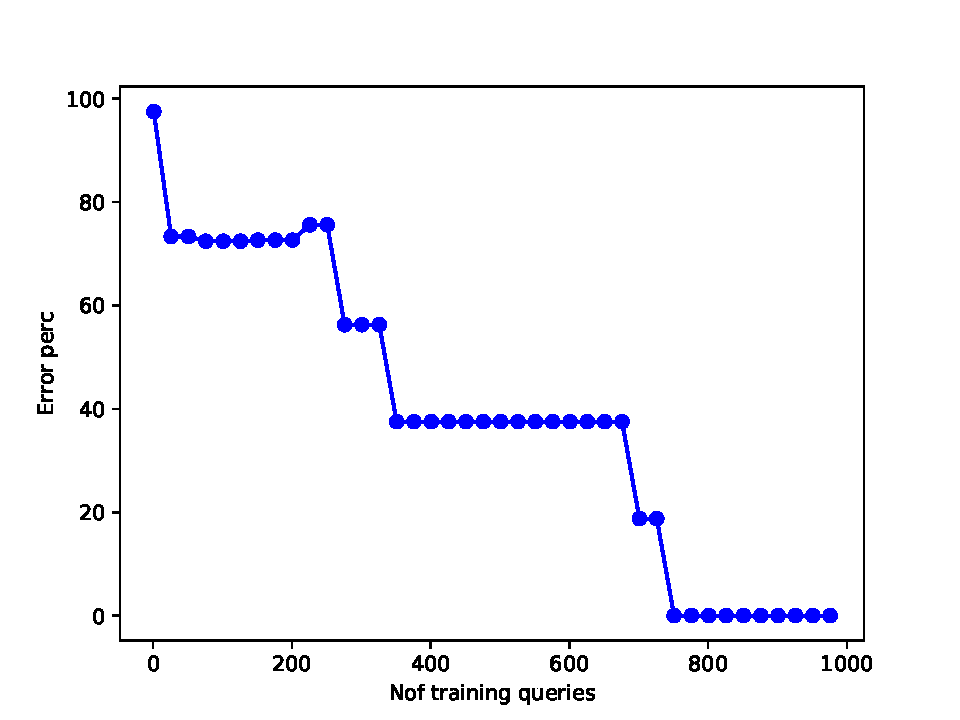
\includegraphics[scale=0.5]{../figs/airtraffic/airtraffic_sel10_error.pdf}
	  %   % \caption{Q10 select error}
	  %   \label{fig:sel04}
	  % \end{subfigure}
	  % \begin{subfigure}[t]{0.4\textwidth}
	  %   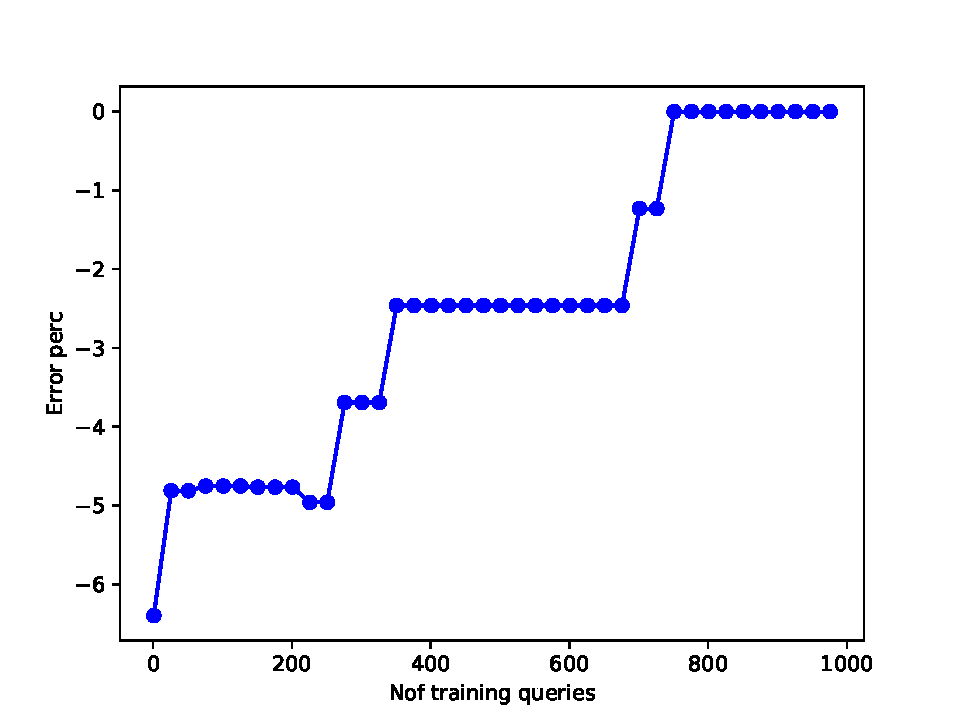
\includegraphics[scale=0.3]{../figs/airtraffic/airtraffic_q10_memerror.pdf}
	  %   \caption{Q10 memory error}
	  %   \label{fig:mem04}
	  %  \end{subfigure}
	\end{figure}
\end{frame}

\begin{frame}[fragile]
% \frametitle{Airtraffic benchmark suite}
\begin{lstlisting}[basicstyle=\ttfamily\footnotesize, language=SQL, escapechar=!]
SELECT *
FROM ontime
!\colorbox{yellow}{WHERE "DepDelay" > 15 AND "ArrDelay" > 15}!
!\colorbox{yellow}{AND "Month" = 3 AND "DayofMonth" = 24 AND "Year" = 2013}!
\end{lstlisting}
	\begin{figure}[!htb]
	    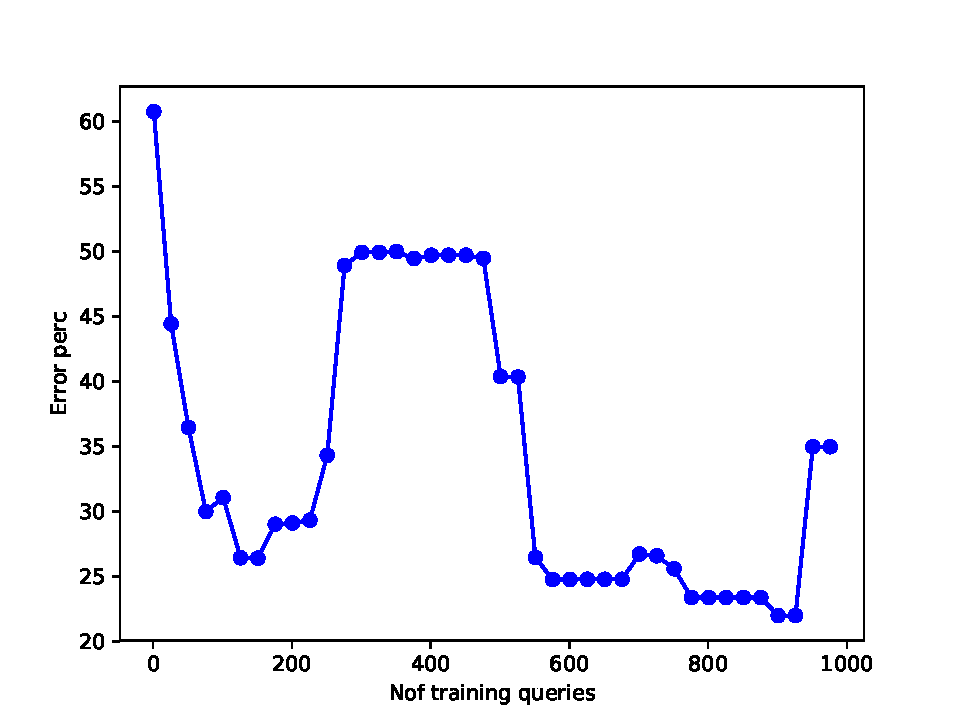
\includegraphics[scale=0.45]{../figs/airtraffic/airtraffic_sel09_error.pdf}
	    \caption{Q09 select error}
	  % \begin{subfigure}[t]{0.4\textwidth}
	  %   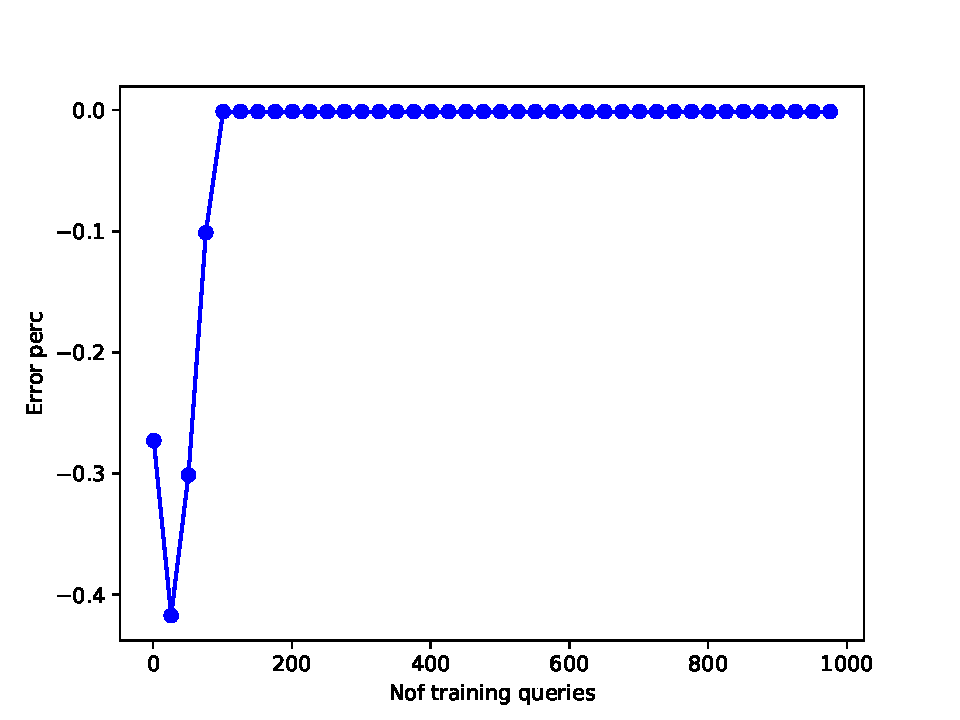
\includegraphics[scale=0.3]{../figs/airtraffic/airtraffic_q09_memerror.pdf}
	  %   \caption{Q09 memory error}
	  %   \label{fig:mem04}
	  %  \end{subfigure}
	\end{figure}
\end{frame}


\begin{frame}[fragile]
\frametitle{Future Work}
\begin{block}{}
\begin{itemize}
\item Provide min,avg,max policies
\item Consider parallel executions
\item Handle correlated columns on selections
\item Also use histograms
\end{itemize}
\end{block}
\end{frame}


\subsection*{Acknowledgments}
This research has received funding from the European Union’s Horizon 2020 research and innovation programme under Grant Agreement no. 732366 (ACTiCLOUD).

{\small
\bibliography{references}
\bibliographystyle{alpha}
}
%\printindex
\subsection*{Appendix}
In this section we collect some user scenarios. screenshots of how it should feel.
and scripts.
